%-------------------------------------------------------------------------------
% midi_export
%-------------------------------------------------------------------------------
%
% \file        midi_export.tex
% \library     Documents
% \author      Chris Ahlstrom
% \date        2018-10-20
% \update      2025-05-15
% \version     $Revision$
% \license     $XPC_GPL_LICENSE$
%
%     This section discusses the details of the import/export functionality.
%
%-------------------------------------------------------------------------------

\section{Import/Export}
\label{sec:midi_export}

   This section explains the details of the MIDI import and export
   functionality, accessed by the main menu as noted in sections
   \ref{subsubsec:menu_file_import},
   \ref{subsubsec:menu_file_export_project},
   \ref{subsubsec:menu_file_export_song_as_midi}, and
   \ref{subsubsec:menu_file_export_midi_only}, on page
   \pageref{subsubsec:menu_file_import}.

\subsection{File / Import Menu}
\label{subsec:midi_export_file_import_menu}

   The actions for importing files have been move to the new
   \textbf{File / Import} menu in order to keep from cluttering the
   ever-expanding file menu.

\subsubsection{Import Project Configuration}
\label{subsubsec:midi_export_file_import_project}

   This operation allows one to import all of the \texttt{qseq66.*}
   configuration files from a given directory into the current run of
   \textsl{Seq66}.
   It is most useful when
   importing a configuration into a new \textsl{NSM} session.
   \index{restart!automatic}
   Once the files are copied, \textsl{Seq66} is automatically restarted,
   in order to load the new configuration.  Be careful!

   Note that the names of the configuration files being impported should
   match the canonical names.  That is, the base names should all be
   \texttt{qseq66} (or \texttt{qpseq66} for \textsl{Windows}.)

   If importing into an NSM session, one must use the NSM user-interface
   (\textsl{agordejo}, \textsl{RaySession}, or \textsl{nsm-legacy-gui}
   to \textsl{Stop} and then \textsl{Start} \textsl{Seq66}.

\subsubsection{Import MIDI to Current Set}
\label{subsubsec:midi_export_file_import}

   The \textbf{File / Import / Import to Current Set} menu entry imports an SMF 0
   or SMF 1 MIDI file as one or more patterns, one pattern per track, and
   imports them into the currently-active set.
   Even long tracks, that aren't short loops, are imported.
   The difference from \textbf{File / Open} is that the destination screen-set
   (bank) for the import can be specified, and the existing data in the
   already-loaded MIDI file is preserved.
   If the imported file is a
   \textsl{Seq66} MIDI file, it's proprietary sections will
   \textsl{not} be imported, in order to preserve the performance setup.
   The \textbf{Import} dialog is similar to the \textbf{Open} dialog.

   When imported, each track, whether music or information,
   is entered into its own loop/pattern box (slot).
   The import operation can handle reasonably complex files.
   When the file is imported, the sequence number for each track is
   adjusted to put the track into the desired screen-set.
   The import can place the imported data into any of the 32 available
   screen-sets.  Quite large songs can be built by importing patterns.

   Import also handles SMF 0 MIDI files.  It parcels out the SMF 0 data
   into sequences/patterns for each of the 16 MIDI channels.  It also puts
   all of the MIDI data into the 17th pattern (pattern 16), in case it is
   needed.  Note that this slot is used no matter which screen-set one imports
   the file into.  Bug, or feature?
   Also note that, since the file information has been modified by the import,
   the user will be prompted to save the file when exiting \textsl{Seq66}.
   Finally, conversion to SMF 1 for SMF 0 files can be disabled using the
   'usr' option \texttt{[user-midi-settings] convert-to-smf-1}.

\subsubsection{Import Playlist}
\label{subsubsec:midi_export_file_import_playlist}

   This operation allows one to copy a playlist and its MIDI files.
   from one directory to another.  It is most useful when
   importing a configuration into a new \textsl{NSM} session.
   Here are the steps it performs:

   \begin{itemize}
      \item Copies the selected playlist file (e.g. \texttt{liveset.playlist})
         into the current configuration directory.
         This directory is one of the following:
         \begin{itemize}
            \item The default "home" directory,
               \texttt{\textasciitilde/.config/seq66}.
            \item A "home" directory specified by the \texttt{--home} option.
            \item The session directory created by \textsl{NSM}.
         \end{itemize}
         For discussion, this directory is called "HOME" or "home".
      \item In HOME, creates a directory called (for example)
         \texttt{playlist/liveset},
         where "liveset" is the base part of the playlist name, as in
         \texttt{liveset.playlist}.
      \item The playlist is opened, parsed, and all of the MIDI tunes specified
         in that file are copied into the new playlist directory, preserving
         the directory directory structure of the original playlist.
      \item The 'rc' file is modified to specify the new playlist,
         specify that it is \texttt{active},
         to specify the new \texttt{base-directory} for all of the tunes,
         and to specify that the playlist will be saved at exit.
      \item Lastly, if not running within NSM, \textsl{Seq66} will be
         \index{restart!automatic}
         \textsl{\textbf{restarted}} automatically to load the new,
         active playlist.
         Within NSM, the user must stop and restart \textsl{Seq66}
         manually in the NSM user-interface.
         Be careful!
   \end{itemize}

\subsection{File / Export Menu}
\label{subsec:midi_export_file_export_menu}

   The actions for exporting files have been moved to the
   \textbf{File / Export} menu in order to keep from cluttering the
   ever-expanding file menu.

   An important point to note is the pattern/channel behavior inherited
   from \textsl{Seq24}.
   When a pattern has a channel specified, all MIDI channel events
   (e.g. Note On/Off) are stamped with that channel when exported.
   This applies to exports to plain MIDI files, song exports, and
   exports to the SMF 0 format.

   If one wants to preserve the channel number for all events in
   a pattern, then one should set the channel to the \textbf{Free}
   value.  See \sectionref{subsec:pattern_editor_first_row}, the section on
   \textbf{Channel Selection}.

   Also note that exporting a song or an SMF 0 file require that the song
   be exportable (see the next section).
   Exporting to a regular MIDI does not have this requirement.

\subsubsection{Export Project Configuration}
\label{subsubsec:midi_export_configuration_export}

   This option allows the various \texttt{qseq66.*} configuration
   files to be copied to another directory.
   This feature is useful for creating an alternate configuration or
   for backing up the current configuration.

   At the present time, any files specified in a play-list are
   \textsl{not} copied.

\subsubsection{Export Song}
\label{subsubsec:midi_export_song_export}

   Thanks to \textsl{Seq32}, exporting song performances (see the
   \textbf{Song Editor}) to standard MIDI format has been added.
   The \textbf{File / Export / Export Song} operation modifies the song in the
   following ways:

   \begin{itemize}
      \item Only tracks (sequences, loops, or patterns)
         \index{exportable}
         that are "exportable" are written.  To be exportable, a
         track must have triggers
         (see \sectionref{subsubsec:concepts_terms_performance})
         present in the \textbf{Song Editor}.
         Also \textsl{in the song editor}, it must \textsl{not be muted}.
      \item Each trigger generates the events, including repeats,
         offset-play of the events, and transposition.
         If there is a gap in the layout
         (e.g. due to an \textbf{Expand} operation in the
         \textbf{Song Editor}),
         then the corresponding gap in the events is exported.
         The result is a track that reconstructs the original
         playback/performance layout of that pattern.
         The events themselves are sufficient to play the performance exactly
         in any MIDI sequencer.
         The triggers are useful for further editing of the song/performance,
         so they are preserved in the triggers \textsl{SeqSpec} section, but
         they cover the whole song.
         The process of consolidating the trigger data is called
         "flattening".
      \item Empty pattern slots between tracks are removed.
      \item No matter what set the original track was in, it ends up in the
         first set; sets are consolidated.
      \item Other additions, such as time signature and tempo meta events, are
         written in the same manner as for a normal \textbf{File / Save}
         operation.
   \end{itemize}

   The \textbf{Export} dialog is similar to the \textbf{Open} dialog;
   one will likely want to change the name of the file so as
   not to overwrite it.
   If there are no exportable tracks, the following message is shown:

\begin{figure}[H]
   \centering 
   \includegraphics[scale=0.65]{main-menu/file/light-menu-file-song-unexportable.png}
   \caption{MIDI File Unexportable}
   \label{fig:midi_export_file_unexportable}
\end{figure}

   Once the file is exported, reopen it to see the results of the export.
   The following figure shows a before and after picture of the export, as
   seen in the song editor.

\begin{figure}[H]
   \centering 
   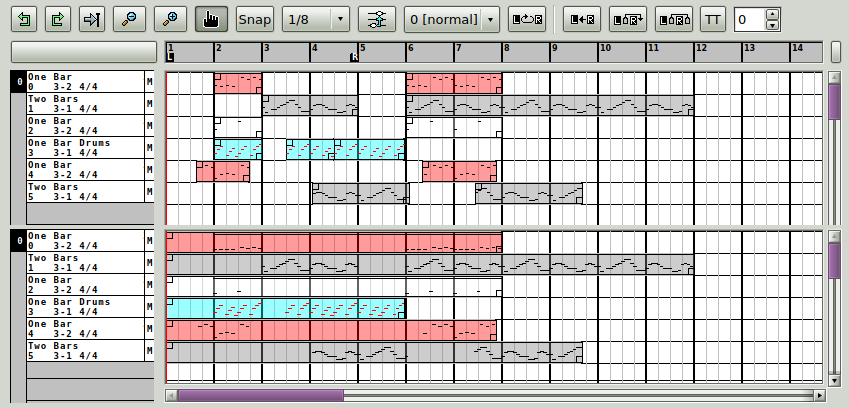
\includegraphics[scale=0.75]{song-editor/song-layout-sample-2.png}
   \caption{MIDI File Layout Before/After Export}
   \label{fig:midi_export_file_before_after}
\end{figure}
   
   The gaps in layouts in the song/performance data are reflected in the
   consolidated triggers.
   Here is the before/after triggers for pattern \#0, which was
   layed out with \textbf{Record Snap} \textsl{on}:

   \begin{verbatim}
       BEFORE                              AFTER
      Sequence #0 'One Bar'               Sequence #0 'One Bar'
      Length (ticks): 768                 Length (ticks): 5375
      trigger: 768 to 1535 at 768         trigger: 0 to 5375 at 5375
      trigger: 3840 to 5375 at 768        
   \end{verbatim}

   Note that 768, at PPQN = 192, is 4 beats (1 measure), while 5375 is 28
   beats (7 measures).
   For each of these triggers, the first number is the start of the trigger in
   PPQNs, the second is the end of the triger, and the third, called the
   "offset", is actually the length of the pattern.
   Note how the "AFTER"
   trigger consolidates the "BEFORE" triggers, starts at time 0, extends to
   the end of the last trigger, and has a length equal to the end of the
   trigger.

   Now here is the before/after triggers for pattern \#5, which was
   layed out with \textbf{Record Snap} \textsl{off}:

   \begin{verbatim}
       BEFORE                              AFTER
      Sequence #5 'Two Bars'              Sequence #5 'Two Bars'
      Length (ticks): 1536                Length (ticks): 6911
      trigger: 2344 to 3879 at 1536       trigger: 0 to 6655 at 6911
      trigger: 4944 to 6655 at 0
   \end{verbatim}

   6655 is a little over 34.5 beats, which is what the bottom grey trigger
   shows.
   6911 is almost 36 beats (9 measures).  Something to figure out.

\subsubsection{Export MIDI Only}
\label{subsubsec:midi_export_file_export_midi_only}

   Sometimes it might be useful to export only the non-sequencer-specific
   (non-SeqSpec) data from a \textsl{Seq66} song.
   For example, some buggy sequencers
   (hello \textsl{Windows Media Player})
   might balk at some SeqSpec item in the song, and refuse to load the MIDI
   file.
   For such cases,
   the \textbf{File / Export / Export MIDI Only} menu
   item writes a file that does not contain
   the SeqSpec data for each track, and does not include all the SeqSpec data
   (such as mute groups) that is normally written to the end of the
   \textsl{Seq66} MIDI file.

\subsubsection{Export SMF 0}
\label{subsubsec:midi_export_file_export_smf_0}

   In some cases it might be useful to convert a \textsl{Seq66} MIDI file to a
   single-track SMF 0 file.
   As with exporting to a song
   (see \sectionref{subsubsec:midi_export_song_export}),
   the tracks to be exported (combined into a single track) must be unmuted
   and have layouts in the song editor.
   The \textbf{File / Export / Export SMF 0 } menu
   action removes all the existing tracks and merges them into track 0.

%-------------------------------------------------------------------------------
% vim: ts=3 sw=3 et ft=tex
%-------------------------------------------------------------------------------
